\chapter{The Bitcoin Network}
	\label{sec:bitcoin}

Bitcoin is a peer-to-peer electronic cash system without any trusted third party and was described by Satoshi Nakamoto in Oktober 2008\cite{nakamoto:bitcoin}. The name Bitcoin refers to both the operating network of nodes and the system's native currency. The network and protocol is usually refereed to with a large B, Bitcoin, and the currency with a small b, bitcoin.\footnote{While it's convention to not capitalize currencies in the English language, it's not widely followed in mainstream or semi-mainstream outlets. Also the plural form of currencies is equivalent to the singular. The convention will be followed in this report.}

\section{Digital Signatures}

Part of the solution is provided by one way asymmetric encryption utilizing the \texttt{secp256k1} elliptic curve. Asymmetric encryption or public-key encryption allows the generation of key pairs with the ability to derive a public key from a private key without the ability to derive the private key from the public key and the ability to prove ownership of the private key through signatures without disclosing the private key. Ownership and expenditure of bitcoin is proved by signing a previous transaction output payable to the public key derived bitcoin address\footnote{A bitcoin address is derived from the public key by hashing the public key with both \texttt{SHA256} and \texttt{RIPEMD160}} with the accompanying private key. 

\begin{figure}[!htb]

	\centering
	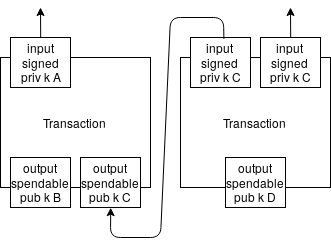
\includegraphics[width=6cm]{images/transaction.png}
	\caption{\textit{A simplified illustration of two transactions. 
	}}
	\label{fig:two:tx}

\end{figure}

Bitcoin is essentially a long ledger of inputs and outputs. Note that the whole output must be spent in the same transaction and usually there is an output leading back to an address the spender controls with the 'change'. The sum of all the inputs and the sum of all the outputs usually does not line up, the differential is the implicit miners fee the miner receives if the transaction is included in a block. 

\section{The Double-Spending problem}

While digital signatures are able prove ownership of bitcoin, there is nothing to stop the owner of an amount of bitcoin to sign two different transactions spending the same transaction output and broadcasting them to different parts of the network. This is called the double-spending problem which is a variation of the more general Byzantine's General Problem.

%\subsection{Proof-of-Work}

The network reaches a coherent global view over the transaction history by a method known as \textit{Proof-of-work}. The Bitcoin \textit{Proof-of-work} algorithm is very similar to that of hashcash as it uses a hash-based cost function which requires a probabilistic amount of work and the proof of the work fixed cost to verify\cite{back:hashcash}\footnote{It's similar to hashcash in both being hash-based with a cost function that is non-interactive, publicly auditable, trapdoor-free and have an unbounded probabilistic cost\cite{back:hashcash}.
Bitcoin uses the double \texttt{SHA256} hash function.}.

The \textit{Proof-of-work} algorithm is directly tied into the bitcoin transaction history data structure composite of a chain of blocks as seen in figure \ref{fig:blockchain}.

\begin{figure}[!htb]
	\hspace*{-0.4cm} 
	\centering
	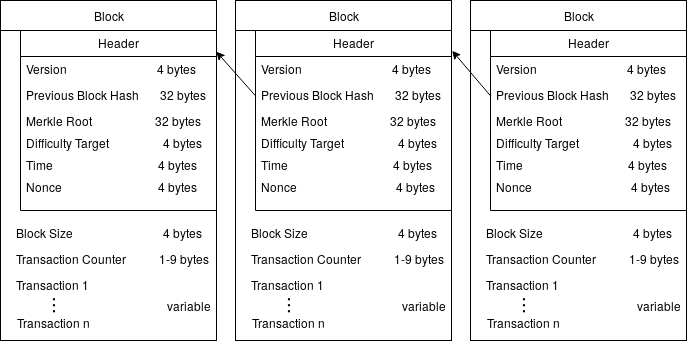
\includegraphics[width=10cm]{images/blockchain.png}
	\caption{\textit{Three blocks linked by the hash of the previous block's header. The content in the header is immutable and can't be replaced without redoing \textit{Proof-of-work}.
	}}
	\label{fig:blockchain}
	\hspace{2mm} 
\end{figure}

The 'work' part of the algorithm is to find a sufficiently small hash of the previous block's header. A hash is valid if it's smaller than a number imposed by a \textit{difficulty target}. There is no way to reverse engineer a sufficient hash and the algorithm repeatedly hashes the block header, changing the nonce, until a hash is found. Consensus is reached by regarding the longest chain of work to be the valid chain. The blocks are in a sense chained through these hashed headers and each additional block adds cumulative work on the blocks below reducing the chance of ever being reverted. The difficulty target adjusts every 2015th\footnote{This is off by one bug, 2016 blocks is two weeks} block\cite{repository:bitcoin} as part of the consensus algorithm and forces the average time between blocks to always be ten minutes. Running the bitcoin \textit{Proof-of-work} algorithm is known as \textit{mining} as per the similarities with the finding and minting of gold coins.

\subsection{Merkle Tree}

\begin{figure}[!htb]
	
	\centering
	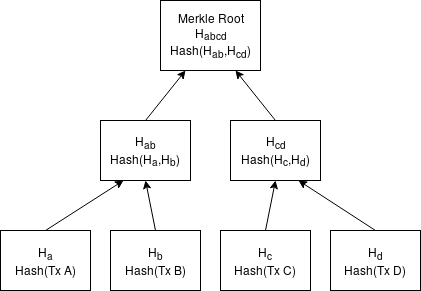
\includegraphics[width=7cm]{images/merkle.png}
	\caption{\textit{A merkle tree resulting from four transactions A, B, C, D.
	}}
	\label{fig:merkle:tree}
	
\end{figure}

The content in the block header is practically immutable since a change would make the hash invalid. The transactions are not in the header but are still immutable by the use of a Merkle tree(see fig \ref{fig:merkle:tree}). A Merkle tree is a binary tree in which the parent is the hash of its two children. The root hash of the tree is included in the header and if any transaction were to change it would also cause the root hash to change rendering each transaction immutable by implication. Bitcoin uses the double \texttt{SHA256} as the Merkle tree hash function.

\subsection{Incentive}

The miners are incentivized by receiving the transaction fees from the transactions included in mined block as well as a subsidy. The subsidy is on the form of a coinbase transaction which has only outputs, this is how new bitcoin is minted. Every fourth year the subsidy halves and by 2140 will be zero. The miner must follow the consensus rules and mined blocks not following the rules will not be propagated through the network causing the miner to loose out on the block reward.

A miner, or a miner cartel, controlling more than 50\% of the hashing power could technically double-spend transactions by mining blocks on a secret chain \textbf{A}, instead of the public chain \textbf{B}, without broadcasting them to the greater network and simultaneously spending outputs \textbf{OB} on chain \textbf{B}. When the chain \textbf{A} is broadcast and if it contains more work than \textbf{B} the outputs \textbf{OB} would be invalidated and never have transpired per the consensus rules. A huge problem with such an attack is that the confidence in the network would decrease causing the value of the 'stolen' bitcoin outputs \textbf{OA} to be close to worthless. The attacker would still own a lot of specialized hardware, only capable of running the \texttt{SHA256} hashing algorithm, that is worthless without utility outside the network. In a sense such an attack would cause mutual destruction for both the network and the attacker. 

\section{Script}
\label{sec:script}

Transactions utilize a forth-like polish-notation stack based execution scripting language\cite{antonopoulos:mastering:bitcoin}. Each transaction output consist of a locking script\footnote{Also refereed to as scriptPubKey. Locking script is a broader term and technically scriptPubKey scripts $ \subseteq $ locking scripts.}. In order to spend an output a valid unlocking script must be provided in the input to the spending transaction that solves the locking script\footnote{scriptSig, witness $\subseteq $ unlocking scripts.}. Validation is performed by executing the unlocking script and locking script sequentially as seen in figure \ref{fig:simple:script}. 

\begin{figure}[!hbt]
		\centering
	\begin{lstlisting}
 <@\texttt{\textcolor{black}{OP\_1}}@>   <@\texttt{\textcolor{black}{OP\_2 OP\_ADD OP\_3 OP\_EQUAL}}@>
<@\texttt{\textcolor{black}{unlock}}@>           <@\texttt{\textcolor{black}{lock}}@>
	\end{lstlisting}
	
	\caption{\textit{ A simple predicate. Evaluated from left to right (1 2 +) -> 3 and
			(3 3 =) -> true. This lock script can obviously be solved by anyone and should not be used with real bitcoin.
	}}
	\label{fig:simple:script}
\end{figure}

The two scripts added together forms a predicate. If the predicate is true the transaction is valid. Nakamoto considered naming the language predicate but went with script to be more inclusive to a broader audience\cite{nakamoto:predicate}.

\subsection{Pay to Public Key Hash}

The Pay-to-Public-key-hash or P2PKH for short was the standard script for a long time. It allows only the owner of 
the private key to the public key to spend the output.

\begin{figure}[!hbt]
		\centering
	\begin{lstlisting}
<@\texttt{\textcolor{black}{<Sig><Pub\_Key>}}@>   
   <@\texttt{\textcolor{black}{unlock}}@>
   
<@\texttt{\textcolor{black}{OP\_DUP OP\_HASH160 <Pub\_Key\_Hash> OP\_EQUALVERIFY OP\_CHECKSIG}}@>
   <@\texttt{\textcolor{black}{lock}}@>
	\end{lstlisting}
	
	\caption{\textit{ The P2PKH locking and unlocking scripts.
	}}
	\label{fig:P2PKH}
\end{figure}

The P2PKH pushes the signature produced by the private key and the public key to the stack. The public key gets duplicated and the top one gets hashed. The \texttt{OP\_HASH160} is a double hash and first hashes the key with \texttt{SHA256} and then \texttt{RIPEMD160}. This is done to hide the public key until expenditure which may be useful if, for example, the ECDSA would break and private keys could be reversed. In the early days of the network this obfuscation technique wasn't used, for example the first transaction between Nakamoto and Finney did not hide the public key\cite{nakamoto:finney:tx}. The \texttt{OP\_EQUALVERIFY} pops the two public key hashes and terminates the script with false if they are not equal. The \texttt{OP\_CHECKSIG} verifies that the signature is indeed a match with the public key and returns true. 

\subsection{Pay to Script Hash}

The Pay-to-Script-Hash or P2SH is a more flexible transaction than the P2PKH and was introduced with BIP016\cite{bip:0016:p2sh}. It allows the locking script to only be the hash of the redeemable script. If a long script with many public keys is considered as seen in figure \ref{fig:cumbersome:script}.

\newpage

\begin{figure}
	\centering
	\begin{lstlisting}
<@\texttt{\textcolor{black}{0 <Sig A> <Sig B>}}@>   
   <@\texttt{\textcolor{black}{unlock}}@>
	
<@\texttt{\textcolor{black}{2 <Pk\_A><Pk\_B><Pk\_C> 3 OP\_CHECKMULTISIG}}@>
   <@\texttt{\textcolor{black}{lock}}@>
	\end{lstlisting}
	
	\caption{\textit{ Showing a multisig transaction which require to two signatures out of three to be spent. Note the \texttt{0} in the unlock script, it's there due to a bug with \texttt{OP\_CHECKMULTISIG} which pops an extra item from the stack. If not for the \texttt{0} it would try to pop an empty stack. The dummy value must be a \texttt{0} with BIP 147 compliant node implementations\cite{bip:0147:dummy:zero}.
	}}
	\label{fig:cumbersome:script}
\end{figure} 

This multisig transaction(in figure \ref{fig:cumbersome:script}) could be rewritten as a P2SH by hashing the locking script with \texttt{SHA256} and  \texttt{RIPEMD160} and utilizing it as seen in figure \ref{fig:p2sh}.

\begin{figure}[hbt!]
	
	\begin{lstlisting}
<@\texttt{\textcolor{black}{0 <Sig A> <Sig B> <redeem script> }}@>   
   <@\texttt{\textcolor{black}{unlock}}@>
	
<@\texttt{\textcolor{black}{OP\_HASH160 <redeem script hash> OP\_CHECKVERIFY}}@>
   <@\texttt{\textcolor{black}{lock}}@>
	\end{lstlisting}
	
	\caption{\textit{ The P2SH transaction which is essentially equivalent to the multisig in figure \ref{fig:cumbersome:script}.
			Note that 'redeem script' corresponds to the lock script in figure\ref{fig:cumbersome:script}.
	}}
	\label{fig:p2sh}
\end{figure}

Converting to a P2SH transaction does two things:

\begin{itemize}

	\item It shifts the fee burden from the sender to the recipient. The locking script is shorter, the unlocking script is longer.
	
	\item All unspent UTXOs must be kept in the RAM of the node, shifting the burden, thus reducing the node RAM load.
	
\end{itemize}

P2SH also allows the script to be used as an address as per BIP013\cite{bip:0013:p2shaddr}. By simply sending to the script address one could potentially fund any type of complex transaction with no added complexity to the sender.

Even though Script is not Turing complete it allows many quite advanced systems on top of it, transactions or output scripts are sometimes referred to as 'smart contracts'\footnote{First formally defined by Nick Szabo in 1994\cite{szabo:smart:contracts}}.

\begin{figure}[hbt!]
	
	\begin{lstlisting}	
<@\texttt{\textcolor{black}{IF }}@>
  <@\texttt{\textcolor{black}{IF }}@>
    <@\texttt{\textcolor{black}{2 }}@>
  <@\texttt{\textcolor{black}{ELSE }}@>
    <@\texttt{\textcolor{black}{<30 days> CHECKSEQUENCEVERIFY DROP}}@>
    <@\texttt{\textcolor{black}{<Pubkey D> CHECKSIGVERIFY}}@>
    <@\texttt{\textcolor{black}{1}}@>
  <@\texttt{\textcolor{black}{ENDIF }}@>
  <@\texttt{\textcolor{black}{<Pk A><Pk B><Pk C> 3 CHECKMULTISIG}}@>
<@\texttt{\textcolor{black}{ELSE }}@>
  <@\texttt{\textcolor{black}{<90 days> CHECKSEQUENCEVERIFY DROP }}@>
  <@\texttt{\textcolor{black}{<Pubkey D> CHECKSIG }}@>
<@\texttt{\textcolor{black}{ENDIF}}@>

	\end{lstlisting}
	
	\caption{\textit{ A more complex multisignature locking script involving timelocks.
	}}
	\label{fig:aantop:multi}
\end{figure}

One example of a more advanced script is this multisignature locking script with timelocks seen in figure \ref{fig:aantop:multi}. The script consists of three clauses, the clause executed is determined by the unlocking script since the condition to \texttt{IF} is the top item on the stack, not the following item as in most languages. The output could be spent by either clause being triggered:
\begin{itemize}
	\item 2 out 3 of the A, B, C signatures.
	\item 30 days passed, D signature and 1 out of A, B, C signatures.
	\item 90 days passed and D signature.
\end{itemize}

\subsection{Relative lock time}
\label{sec:rlt}

The script(figure \ref{fig:aantop:multi}) uses a construction known as a relative time lock and uses the \texttt{OP\_CHECKSEQUENCEVERIFY} opcode in the bitcoin scripting language\cite{bip:0068:sequence:lock:time}. The relative lock time will only become true after the defined time since the parent transaction was included in a block has passed. To avoid the block miners to become oracles of time, the median time of the eleven last blocks are used as the lock time(BIP113\cite{bip:0113:median:time:passed}). The \texttt{OP\_CHECKSEQUENCEVERIFY} was activated by BIP112\cite{bip:0112:sequence:lock:time:soft:fork}. The block time is therefor approximately an hour behind real time.

The Lightning Network utilize many complex transactions and more will be seen in chapter \ref{sec:lightning:network}.

\section{Network}

The Bitcoin network consists of nodes complying with the consensus protocol. In the beginning only the reference implementation available but with the growth of popularity others have implemented independent implementations\cite{repository:bitcoin}\cite{repository:btcd}\cite{repository:neutrino}.

The mining component of nodes has mostly been decoupled from ordinary nodes with the advent of ASIC\footnote{Application Specific Integrated Circuit, hardware that is built only to run \texttt{SHA256}}. Mining nodes still do everything as an ordinary node does as it needs the transaction history to construct valid block. Non mining nodes validates and propagates blocks and transactions across the network. It allows some benefits in constructing transactions but mainly allows the operator to validate that the network operates as expected instead of trusting that it does.

Construction of transactions can be possible without running a node and many bitcoin wallets do not operate as a node.

 

